\documentclass{scrartcl}
\usepackage[utf8]{inputenc}
\usepackage{hyperref}
\usepackage{url}
\usepackage{natbib}
\usepackage{graphicx}
\usepackage{float}
\usepackage{listings}
\usepackage{xcolor}
\usepackage{booktabs}
\usepackage{amsmath}


\usepackage{cleveref} % this must be the last package to be loaded

\title{\LARGE
  Poool Game
}
\subtitle{Concurrent and Distributed Programming\\a.y. 2025--2026}

\author{
    Buda Marco \and Merighi Daniele \and Turchi Jacopo
}

\date{\today}

\begin{document}

\maketitle

\section{Problem Analysis}

This section provides an analysis of the \texttt{Poool} game from a concurrent programming perspective. The main computational challenge resides in the simulation loop, which must continuously handle physics updates, boundary collisions, and elastic collisions among thousands of small balls.

The primary bottlenecks identified are:
\begin{itemize}
    \item \textbf{Linear State Updates:} Modifying positions and applying friction coefficients across large arrays of entities.
    \item \textbf{$O(n^2)$ Collision Resolution:} The nested loop required to evaluate and resolve simultaneous impacts between every pair of balls represents the highest density of CPU cycles.
\end{itemize}

\section{System Architecture and Architectural Design}
This section describes the high level structure of our proposed solution, focusing on the elements of concurrent programming, i.e. the active and passive components at play and their interactions. Visual formalisms, specifically Petri nets, are also used to demonstrate the overall behavior and to allow for preliminary model checking.

\subsection{Parallelization Strategy}
Having identified that the physics simulation represents the most taxing part of the program's computation, it will be the focus of our parallelization efforts. Since it is a CPU-bound problem, the goal will be to distribute the work evenly across all logical processors.

Our solution involves a number of worker threads, handled manually in the Thread-Oriented version, and encapsulated by a \texttt{FixedThreadPool} executor in the Task-Oriented version. We have opted for long-living worker threads, implementing Agenda parallelism, which removes any thread creation overhead.

Every simulation step consists of three phases: updating ball positions, detecting balls inside holes, resolving collisions. The first two phases are linear in the number of balls, thus it is easy to distribute the work evenly, while the collision phase involves $n(n-1)/2$ checks, requiring a more careful approach.

We have decided to view the problem as a triangular matrix, having the rows alternate which worker they are assigned to, as depicted in \Cref{fig:collision_parallelization}. For a large number of balls, this makes for a sufficiently even partition.

\begin{figure}[H]
    \centering
    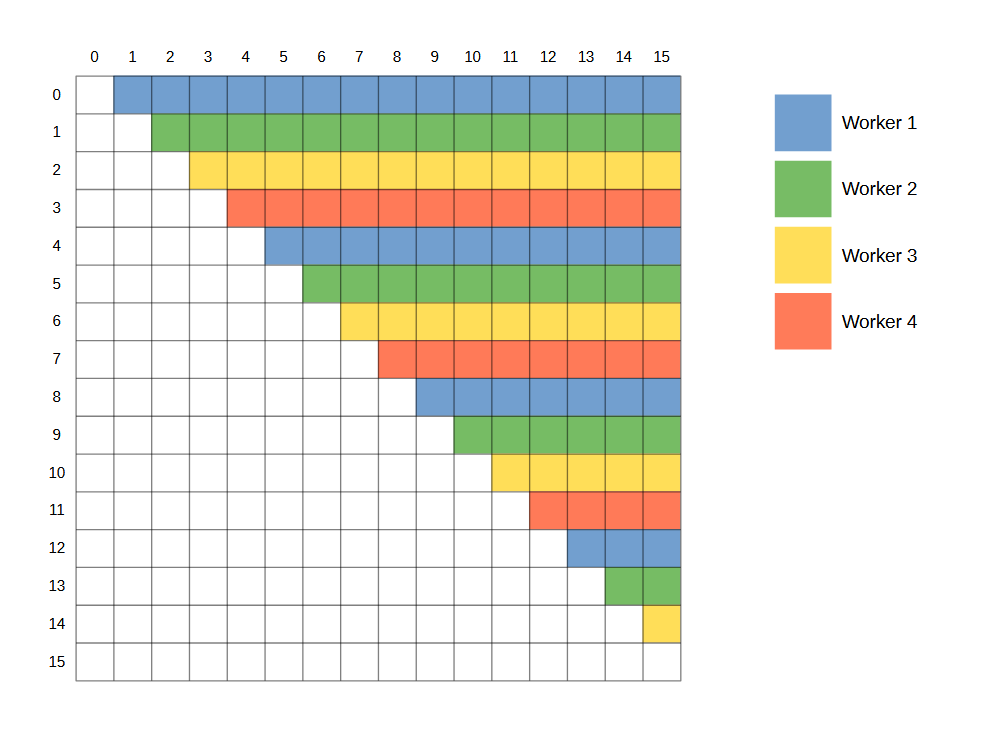
\includegraphics[width=0.6\textwidth]{images/collision_parallelization.png}
    \caption{Matrix representation of the collision resolution phase, showing how the work is partitioned.}
    \label{fig:collision_parallelization}
\end{figure}

\subsection{Active Components}
The concurrent program's execution involves instances of five active classes, each encapsulating a designated control flow.
\begin{itemize}
\item \texttt{KeyboardController}, responsible for the execution of issued keyboard commands, keeping the Graphical User Interface responsive.
\item \texttt{BotUpdater}, periodically kicking the bot player's ball.
\item \texttt{SimulationCoordinator}, distributing the computation for the  physics simulation.
\item \texttt{SimulationWorker}, which performs an assigned portion of the simulation workload. In the Task-Oriented version it is replaced simply by \texttt{java.lang.Thread} and managed by the Java Executor framework. In both cases, multiple instances are expected to be active during the game's runtime.
\item \texttt{java.awt.EventDispatchThread}, provided by Java Swing, which handles graphical events.
\end{itemize}

\subsection{Monitors}
All active components are implemented to be pure, meaning that interactions between them happen through the use of synchronized passive components. Our solution makes use of five such classes.
\begin{itemize}
\item \texttt{BoundedBuffer}, used as the keyboard command buffer.
\item \texttt{Latch}, handling synchronization between the simulation coordinator and workers in the Thread-Oriented version.
\item \texttt{SynchCell}, used to assign work to individual workers in the Thread-Oriented version.
\end{itemize}
Of these, \texttt{BoundedBuffer} and \texttt{Latch} are implemented following the standard semantics, while \texttt{SynchCell} features an additional \texttt{end()} method, which is used to signal that no more values will be put into the cell. This also wakes up all threads that happen to be blocked on the \texttt{get()} method, causing an empty \texttt{Optional} to be returned.
\begin{itemize}
\item \texttt{GameState}, a custom component encapsulating the game's mutable state, including the current list of small balls and the player scores.
\item \texttt{Ball}, which is made into a monitor so that worker threads are competing for resources as rarely as possible.
\end{itemize}

\subsection{Behavior Overview}
We use Petri nets to show a simplified view of the program's information flow. At this level of abstraction the events are atomic, due to all monitor procedures being marked as \texttt{synchronized}. This also means that the mutual exclusion to these objects doesn't need to be depicted explicitly, focusing instead on the more high level constructs.

\begin{figure}[H]
    \centering
    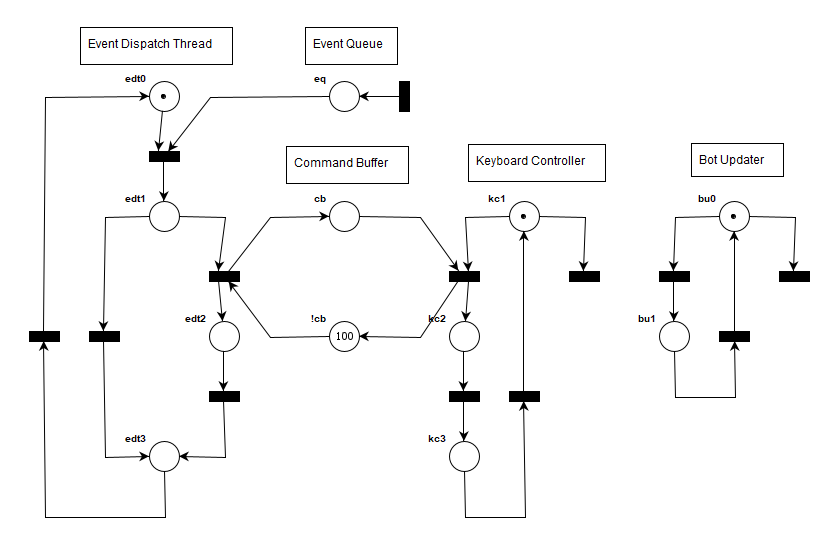
\includegraphics[width=0.9\textwidth]{images/petri_net_1_edt_kc_bu.png}
    \caption{Petri net for the interactions between the Event Dispatch Thread, Keyboard Controller, and Bot Updater active instances.}
    \label{fig:petri_net_1_edt_kc_bu}
\end{figure}

\Cref{fig:petri_net_1_edt_kc_bu} shows an approximation of the control flow within Java Swing's Event Dispatcher Thread, which repeatedly gets events from the Event Queue and executes them. In the case of a keyboard event, the registered callback issues a keyboard command to the command buffer.

The Keyboard Controller follows a similar logic, getting commands from the buffer and executing them within the game's context, until the game ends.

The Bot Updater is autonomous, consisting only of a periodic interaction with the bot player's ball, likewise stopping once the game ends.

\begin{figure}[H]
    \centering
    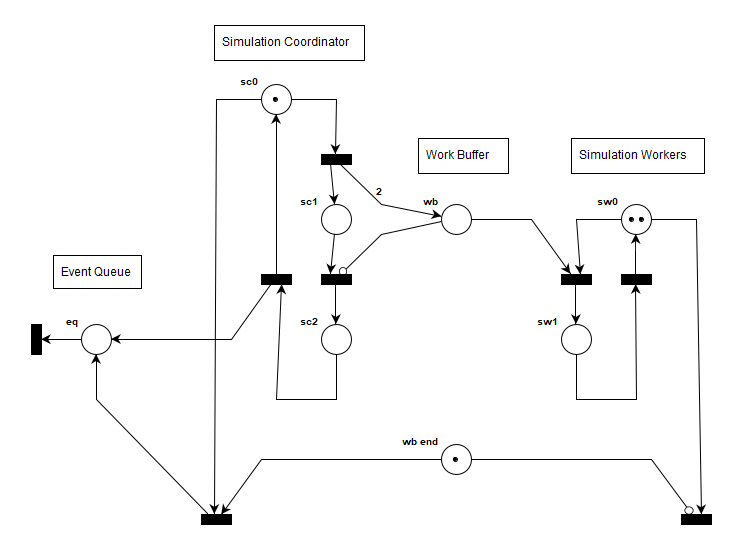
\includegraphics[width=0.8\textwidth]{images/petri_net_2_sc_sw.png}
    \caption{Petri net for the interactions between the Simulation Coordinator and Workers active instances.}
    \label{fig:petri_net_2_sc_sw}
\end{figure}

\Cref{fig:petri_net_2_sc_sw} shows how the physics simulation is parallelized, using two designated workers in this example.

At every iteration, the coordinator divides the workload and assigns it to the work buffer. In the Thread-Oriented version, this buffer is implemented as a list of synchronized cells, so that the workers are not competing for a single object, alongside a latch which is used to detect when all threads have completed their assigned work. In the Task-Oriented version, the same is achieved by making use of the \texttt{executorService.invokeAll()} method.

The workers simply wait for work on their respective cell, calling \texttt{latch.coundDown()} upon completion.

At every iteration, the coordinator may determine that the game is over. In the Thread-Oriented version, this is done by calling the \texttt{synchCell.end()} method for all workers, so that they are allowed to terminate. In the Task-Oriented version, the coordinator simply calls \texttt{executorService.shutdown()}.

As is shown, each simulation step, as well as the game's ending, generates an event to be processed by the Graphical User Interface. The event is added to the Event Queue by means of the \texttt{SwingUtilities.invokeLater()} method.

\subsection{Transition Analysis}
The reported Petri nets were analyzed using the Platform Independent Petri net Editor (PIPE). The reachability graph is shown to contain a single marking with no active transition, which happens to be the state in which all threads have terminated. Because of this, we can assert that the proposed solution is correct and free of deadlocks.

\section{Performance Evaluation}
This section evaluates the empirical performance gains of the concurrent implementations compared to the baseline sequential approach under heavy workloads.

\subsection{Methodology}
Testing was conducted utilising the \texttt{MassiveBoardConf} configuration (4500 entities) to generate a compute-intensive workload. To ensure measurement accuracy, the physics and collision resolution logic \texttt{updateState()} was isolated. The GUI was disabled to eliminate the interference of the sequential Swing event dispatch thread.

Execution times were recorded using \texttt{System.nanoTime()}. Each configuration executed a 1000-update warm-up phase to allow the JVM Just-In-Time (JIT) compiler and Garbage Collector to stabilise, mitigating dynamic compilation overhead as described in ``Performance of Concurrent Programs'' slides. The following 2000 updates were measured, and the average execution time was calculated across 5 independent runs per configuration.

The baseline sequential execution time ($T_{seq}$) averaged 105.65ms per frame for the task version and 106.17ms for the thread one. The host system for the benchmark featured 12 available logical processors ($N_{cpu} = 12$).

\subsection{Concurrent vs. Sequential Advantage}
To evaluate how much the concurrent version improves upon the sequential one, Speedup ($S$) was calculated using the formula $S = T_{seq} / T_N$, where $T_N$ is the execution time with $N$ workers.

\begin{table}[H]
    \centering
    \begin{tabular}{@{}lcccc@{}}
        \toprule
        \textbf{Workers} & \textbf{Task Time} & \textbf{Thread Time} & \textbf{Task Speedup} & \textbf{Thread Speedup} \\
        & \textbf{(ms)} & \textbf{(ms)} \\ \midrule
        1 & 105.65 & 106.17 & 1.00x & 1.00x \\
        2 & 55.96 & 56.76 & 1.89x & 1.87x \\
        4 & 30.48 & 30.92 & 3.47x & 3.43x \\
        8 & 23.11 & 23.51 & 4.57x & 4.52x \\
        \textbf{12} & \textbf{16.74} & \textbf{18.31} & \textbf{6.31x} & \textbf{5.80x} \\
        13 & 21.92 & 22.67 & 4.82x & 4.68x \\ \bottomrule
    \end{tabular}
    \caption{Average execution time and Speedup for Task-Oriented and Thread-Oriented architectures.}
    \label{tab:speedup}
\end{table}

The empirical data demonstrate a definitive advantage of concurrent execution. The Task-Oriented implementation (utilising the Executor framework) achieves a peak speedup of 6.31x at 12 workers, reducing the frame computation time from 105.65 ms to 16.74 ms. The Thread-Oriented architecture yields a similar peak speedup of 5.80x (18.31 ms). This confirms that distributing the physics workload across multiple active components substantially accelerates execution compared to the sequential variant.

\subsection{Core Exploitation and Scalability}
To assess how effectively the program exploits available cores, Efficiency ($E$) was calculated using the formula $E = S / N$.

\begin{table}[H]
    \centering
    \begin{tabular}{@{}lcc@{}}
        \toprule
        \textbf{Workers} & \textbf{Task Efficiency} & \textbf{Thread Efficiency} \\ \midrule
        1 & 1.00 & 1.00 \\
        2 & 0.94 & 0.94 \\
        4 & 0.87 & 0.86 \\
        8 & 0.57 & 0.56 \\
        \textbf{12} & \textbf{0.53} & \textbf{0.48} \\
        13 & 0.37 & 0.36 \\ \bottomrule
    \end{tabular}
    \caption{Computational Efficiency scaling per worker count.}
    \label{tab:efficiency}
\end{table}

\begin{figure}[H]
    \centering
    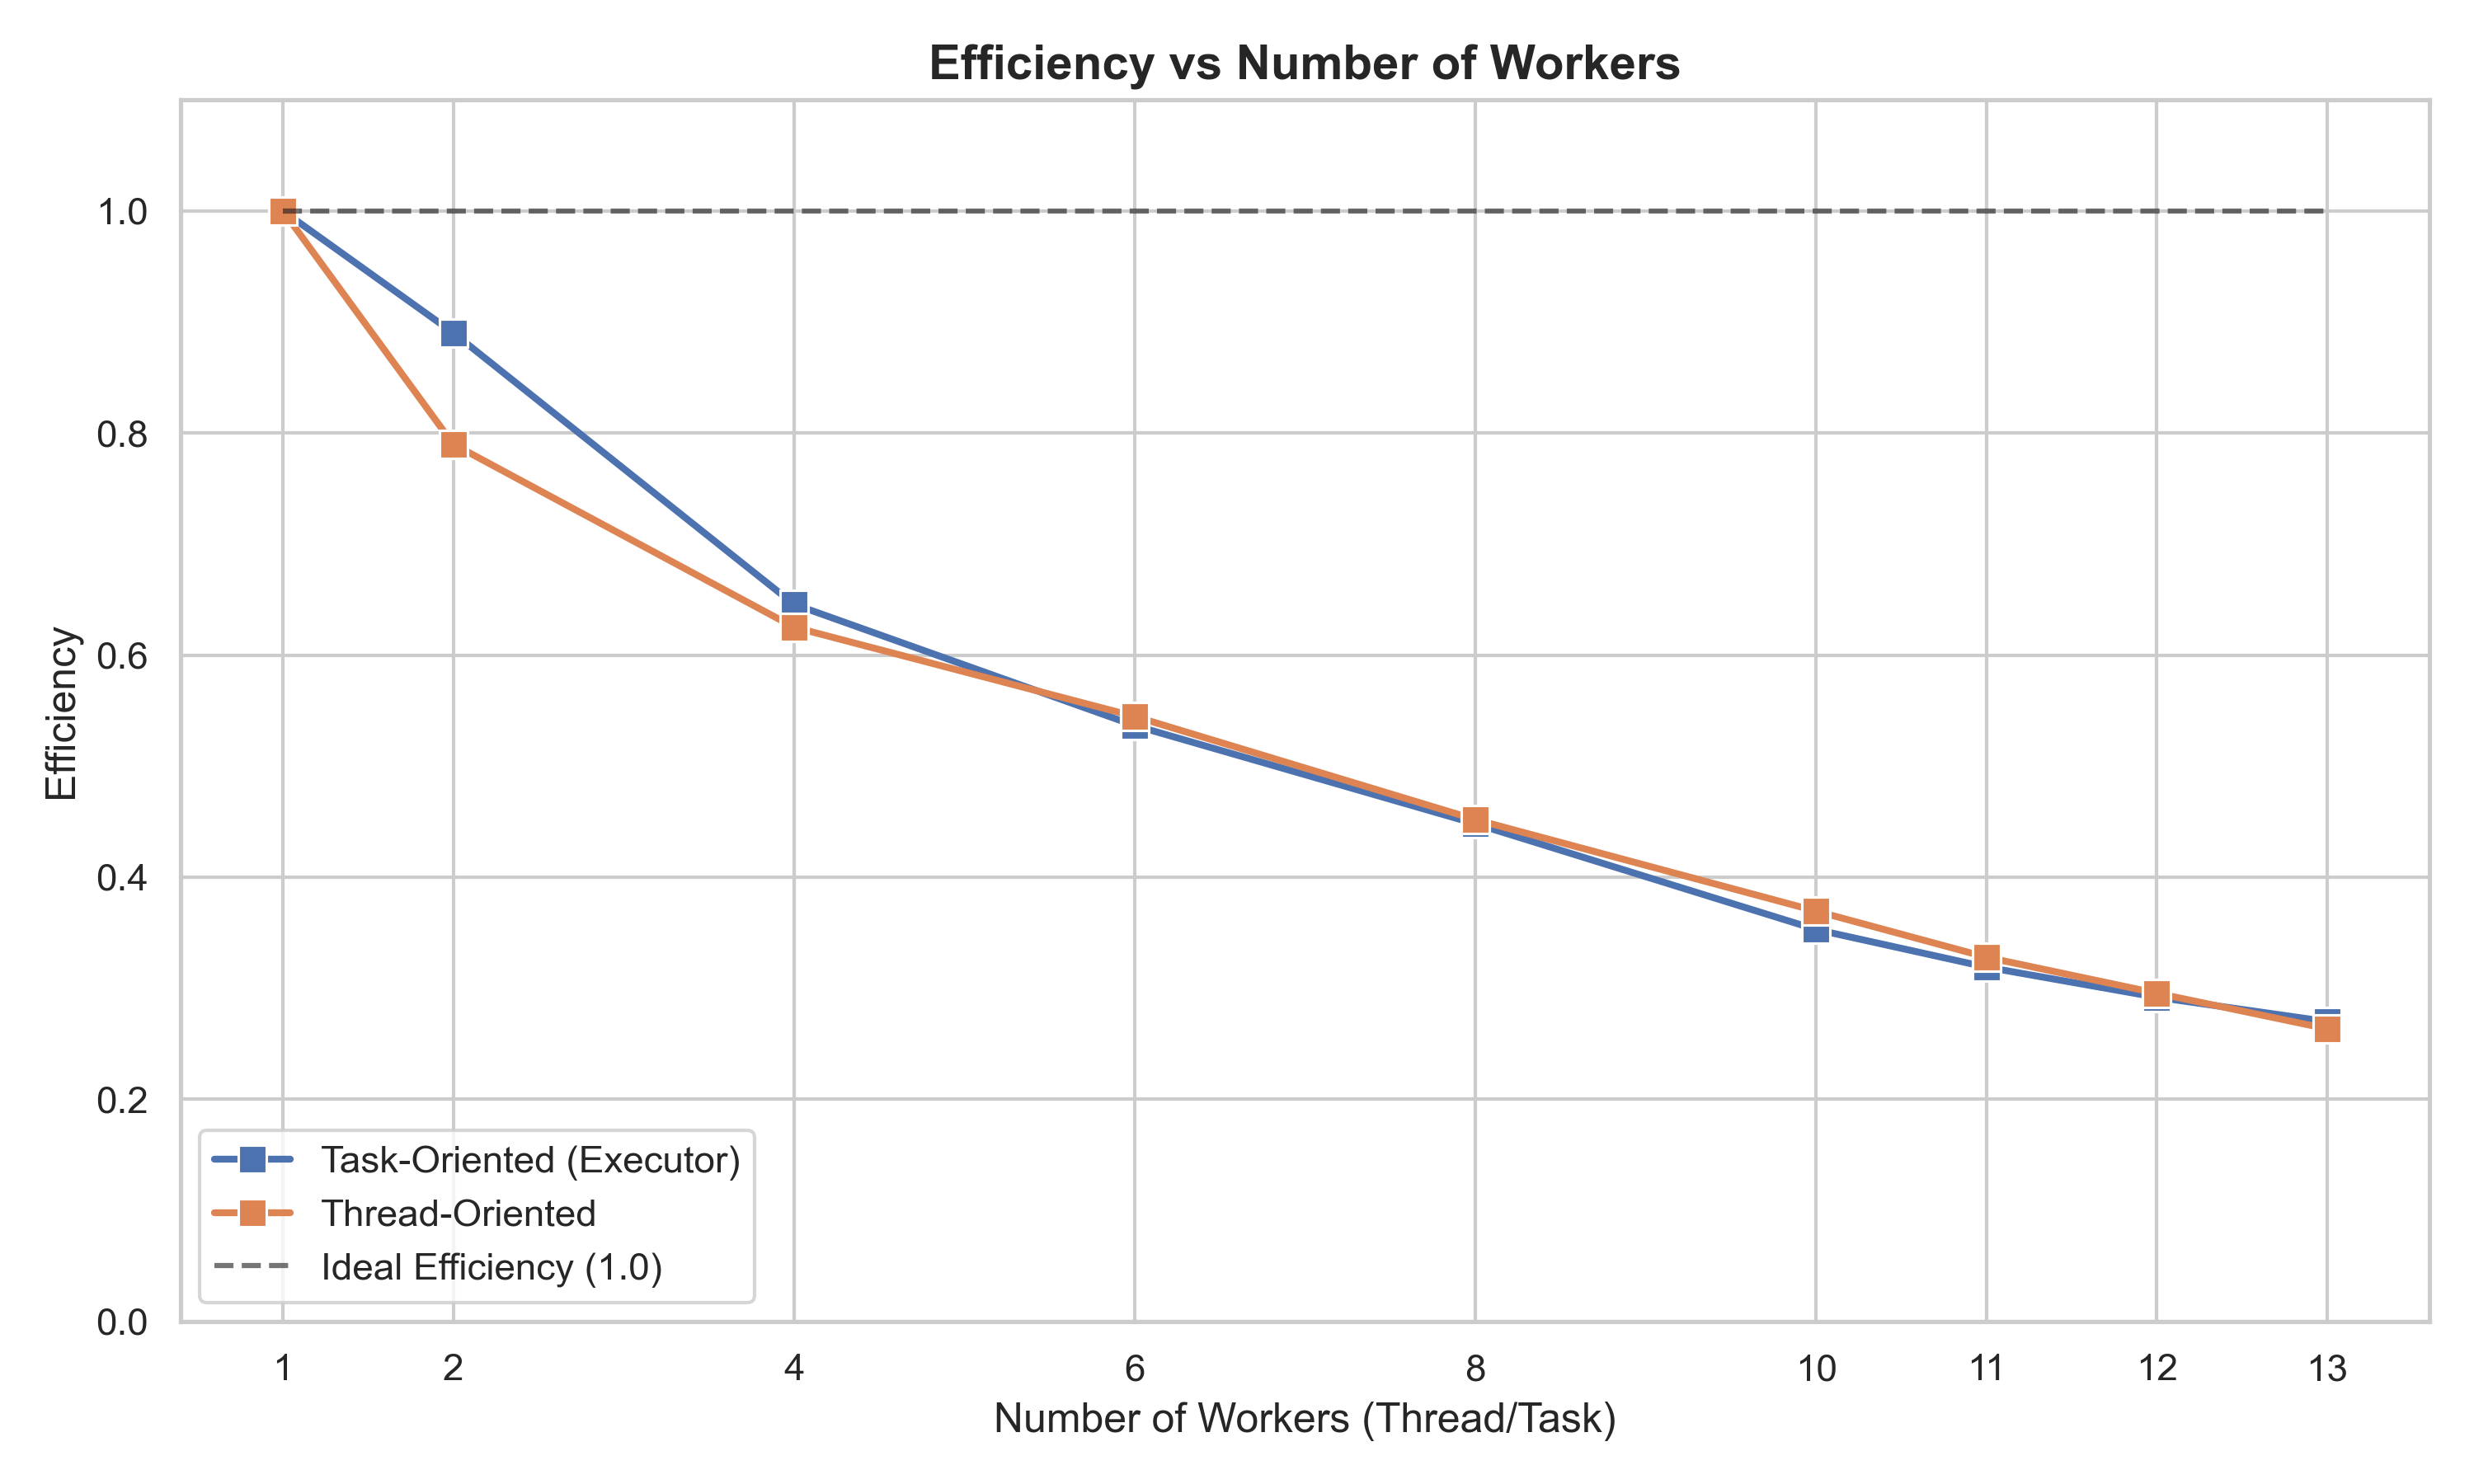
\includegraphics[width=0.9\textwidth]{images/efficiency_plot.png}
    \caption{Efficiency decay.}
    \label{fig:efficiency_plot}
\end{figure}

The application exhibits high efficiency ($> 86\%$) when scaling from 1 to 4 workers. The computation-heavy nature of the collision detection algorithm allows the processors to be exploited directly with minimal synchronisation penalties.

However, efficiency decays as the worker count increases. At 8 workers, efficiency drops to 57\%, and at the $N_{cpu}$ limit of 12 workers, it falls to 53\% (Task-Oriented). This sub-linear scaling is caused by multithreading costs, specifically context switching and lock contention over the shared structures tracking the game state.

Testing with 13 workers ($N_{cpu} + 1$) caused a performance regression. While deploying $N_{cpu} + 1$ threads is a standard heuristic to prevent CPU cycle waste during page faults, the collision resolution task is strictly CPU-bound without blocking I/O operations. Consequently, oversubscribing the CPU forced thread scheduling overhead, dropping efficiency below 40\%.

Overall, the Task-Oriented framework proved slightly more effective at exploiting cores than the Thread-Oriented approach, maintaining lower structural overhead per unit of work distributed.

\subsection{Theoretical Limits and Amdahl's Law Analysis}

\begin{figure}[H]
    \centering
    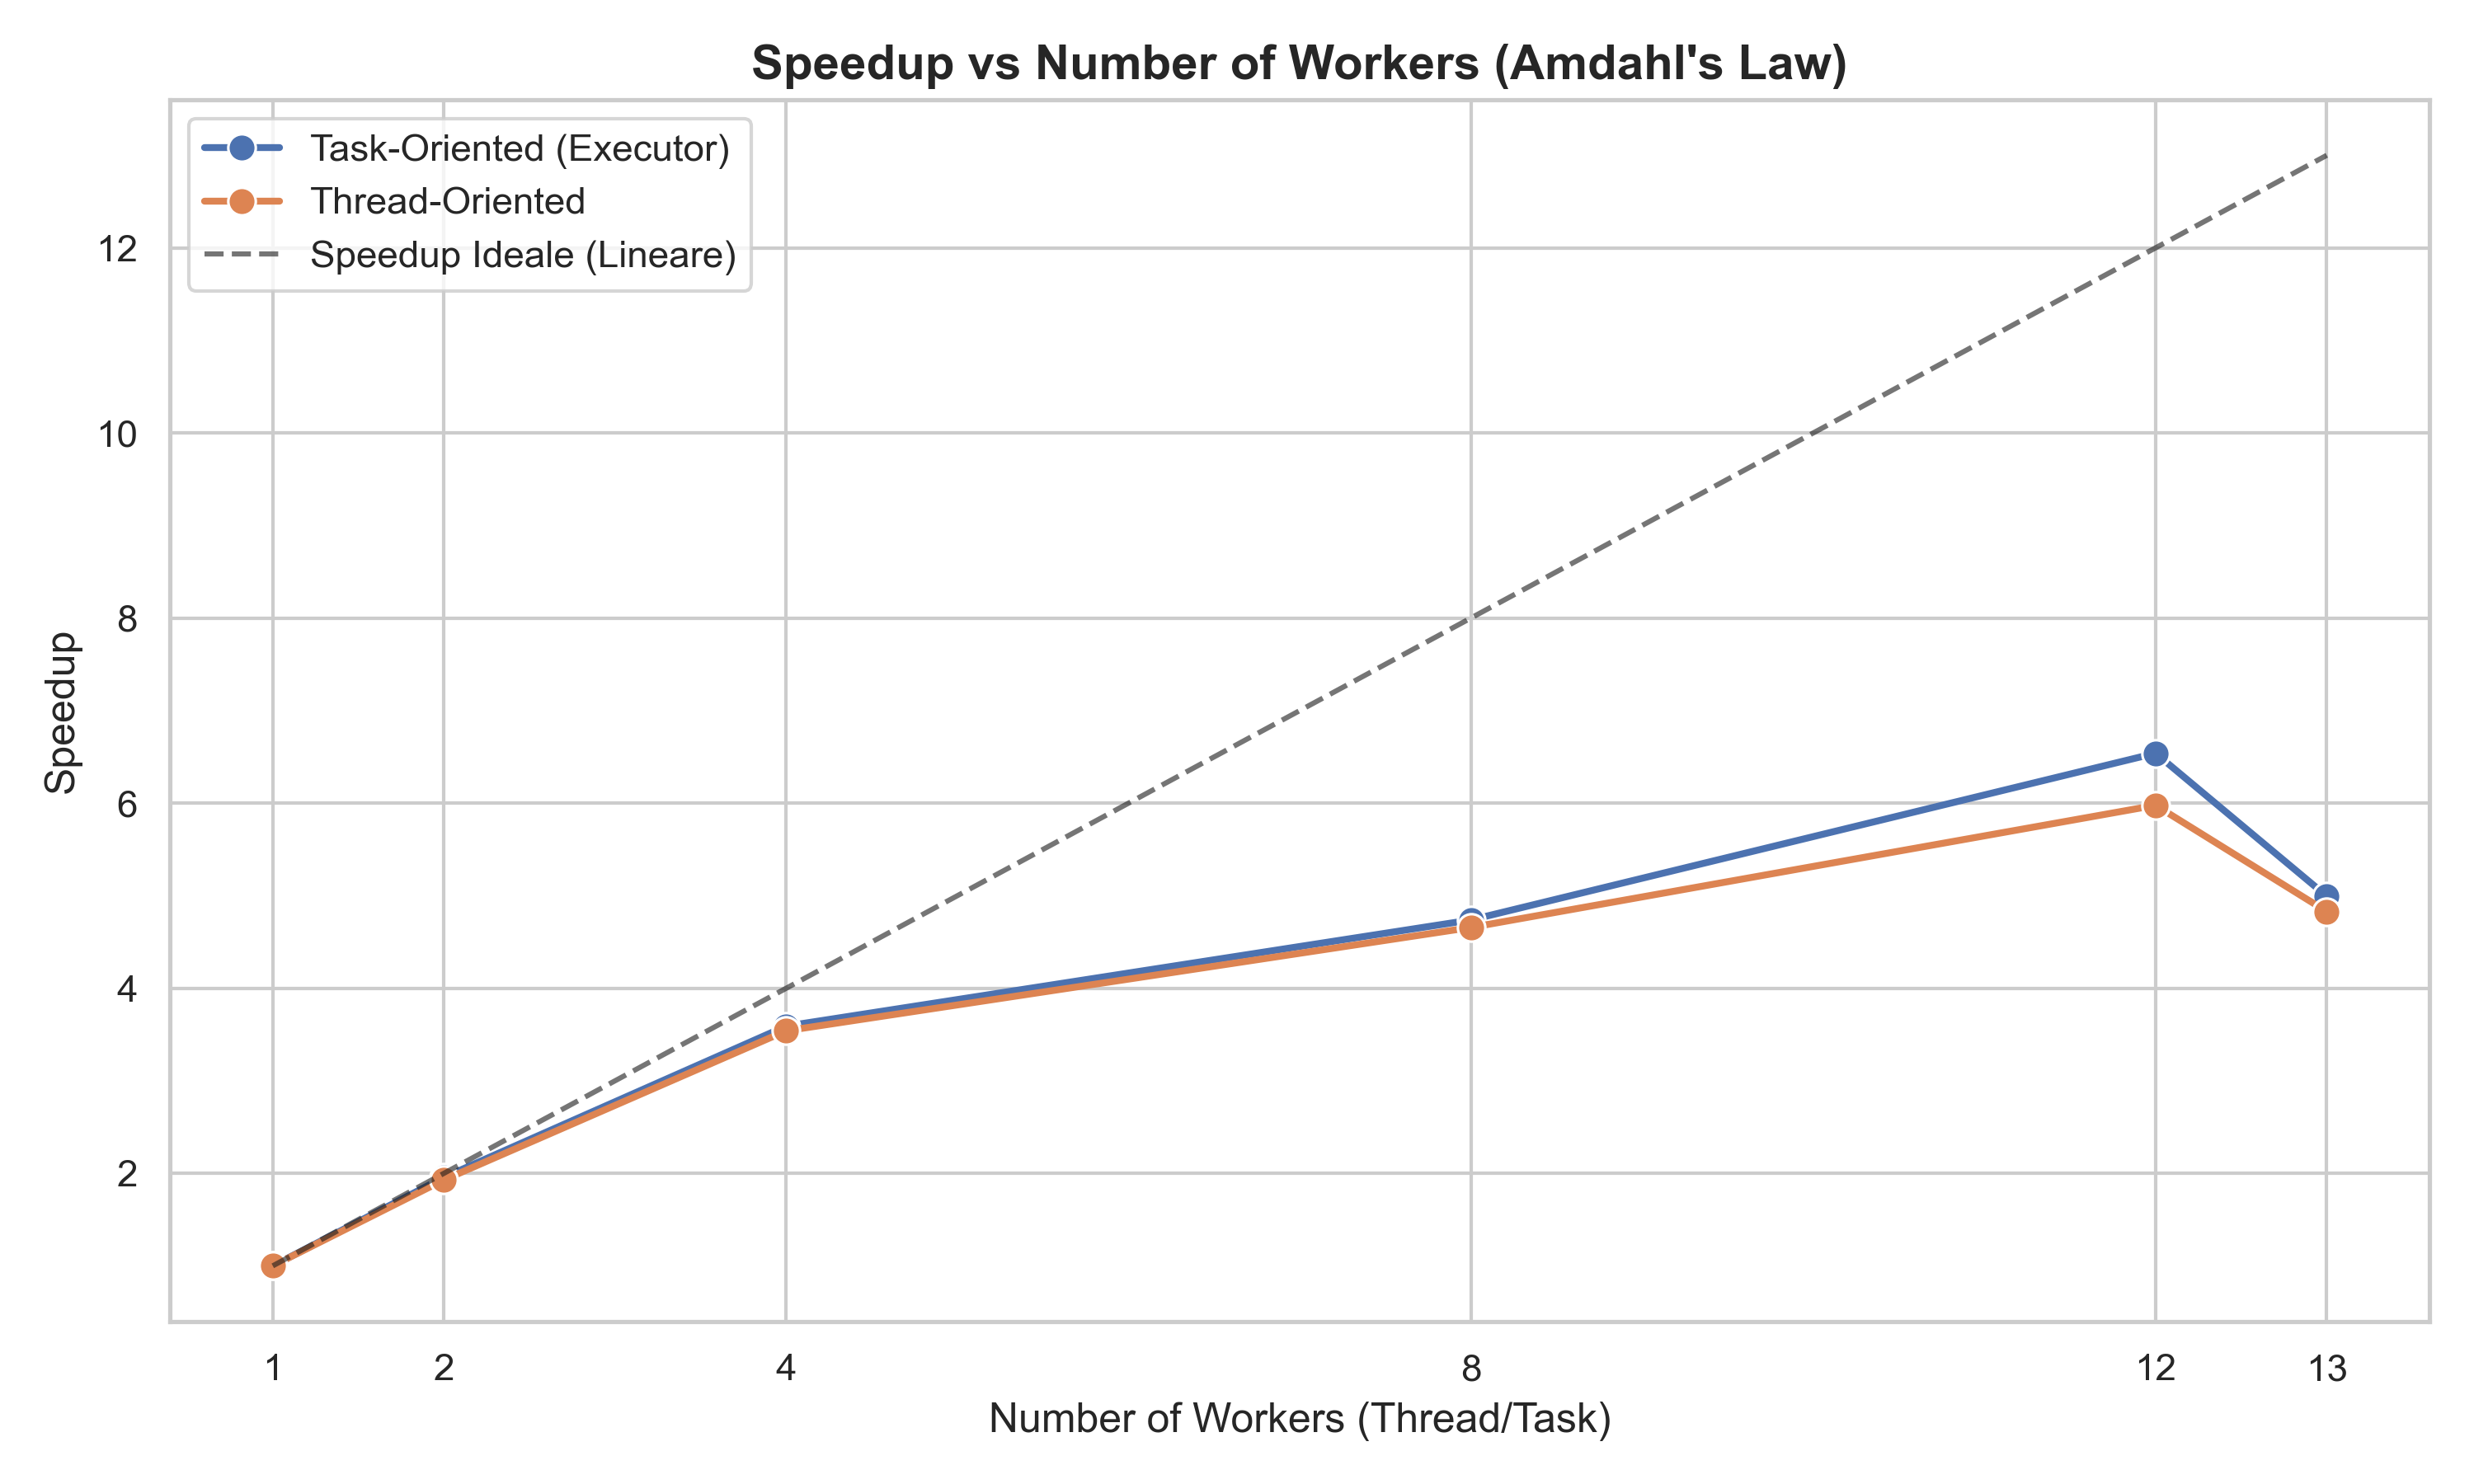
\includegraphics[width=0.9\textwidth]{images/speedup_plot.png}
    \caption{Speedup scaling compared to the ideal linear trajectory.}
    \label{fig:speedup_plot}
\end{figure}

To mathematically contextualise the deviation from the ideal linear speedup shown in Figure \ref{fig:speedup_plot}, Amdahl's Law is applied. This principle states that the maximum achievable speedup is strictly bounded by the fraction of the algorithm that can be made parallel (P)

Using the peak empirical speedup ($S = 6.31$) achieved with $N = 12$ workers in the Task-Oriented architecture, the exact sequential and parallelizable ($P$) proportions of the application can be derived:
$$ S = \frac{1}{1 - P + \frac{P}{N}} \implies 6.31 = \frac{1}{1 - P + \frac{P}{12}} $$
Solving for $P = \frac{5.31 \times 12}{6.31 \times 11}$, it is determined that the highly parallelizable portion of the program is $P \approx 0.918$ ($91.8\%$).

\begin{itemize}
    \item \textbf{The Parallelizable $91.8\%$:} This vast majority of execution time is successfully distributed across the worker pool. It comprises the $O(n^2)$ nested loop evaluating elastic collisions and the linear passes updating entity positions and resolving boundary bounces.
    \item \textbf{The Sequential $8.2\%$ (The Bottleneck):} This unscalable fraction prevents the application from reaching ideal efficiency. Code analysis of the \texttt{Simulation Coordinator} isolates this bottleneck to:
    \begin{itemize}
        \item \textbf{Barrier Synchronization Overhead:} The coordinating thread must block and wait for all workers to complete their discrete tasks via \texttt{invokeAll(work)} or \texttt{Latch.await()} before proceeding to the next frame computation step.
        \item \textbf{Centralized State Evaluation:} Operations such as checking \texttt{isGameOver()} and verifying if any small balls remain are inherently sequential and execute solely on the primary thread, even if some worker would be ready for more work.
        \item \textbf{Loop and Timing Mechanics:} System clock polling and FPS calculations executed within the main \texttt{while} loop contribute to the baseline serial execution cost.
    \end{itemize}
\end{itemize}
This $8.2\%$ structural bottleneck accurately explains why the efficiency curve decays from $94\%$ at 2 workers to $53\%$ at 12 workers, visually validating the theoretical limits predicted by Amdahl's Law.

\section{Program Verification and Model Checking}

This section reports the formal verification of the simulation logic with Java PathFinder (JPF), an explicit-state model checker that explores all the thread interleavings of a Java program. The goal was to confirm the absence of data races and deadlocks in both concurrent architectures.

\subsection{Methodology and Verification Target}

JPF supports only Java 11 and does not scale to arbitrary program sizes, because its state space explodes with the number of threads and synchronisation events. Direct verification of the production code was not possible. A minimal variant \texttt{pooolThreadOrientedJpf} was therefore built, faithful to \texttt{pooolThreadOriented} except where strictly required.

The view, the keyboard controller, the board observers, and the \texttt{BotUpdater} were removed to keep the state space tractable for JPF. \texttt{BotUpdater} also relied on \texttt{java.util.Random}, which JPF treats as an unbounded non-deterministic choice generator. \texttt{Record} declarations and \texttt{switch} expressions were rewritten in pre-Java 14 form. The lambdas inside \texttt{distributeWork} were replaced with anonymous inner classes, because JPF historically does not handle \texttt{invokedynamic} reliably. A bounded counter \texttt{maxTicks} was added to the coordinator to guarantee termination, as JPF requires the program to halt before it can certify any property. A constant tick interval replaced \texttt{System.currentTimeMillis()}, which under JPF does not advance.

The collision phase now uses a spatial grid. Its production size (150 cells) made even the two-ball base run run out of memory, so for JPF the cell size was enlarged with a single constant (\texttt{maxRadius} from $0.1$ to $0.5$), reducing the grid to 6 cells. This loses no collisions, because the balls are far smaller than a cell, and still keeps both workers busy in the collision phase.

The base configuration used \texttt{MinimalBoardConf}, two workers, and two ticks. The listener \texttt{PreciseRaceDetector} was active in addition to the default \texttt{NotDeadlockedProperty}.

\subsection{Race Condition on Ball Position}

The first violation raised by JPF was a data race on \texttt{Ball.pos}. The opening lines of \texttt{Ball.resolveCollision} accessed \texttt{a.pos} and \texttt{b.pos} as direct fields, while the writes always go through the \texttt{synchronized} accessors of \texttt{Ball}. Under the Java Memory Model this counts as a race, and \texttt{PreciseRaceDetector} flagged it. The fix was to read \texttt{pos} and \texttt{radius} through the existing getters at the entry of the method, so that every access happens under the same monitor as the writes. The same change was backported to the production \texttt{pooolThreadOriented} and \texttt{pooolTaskOriented}.

\subsection{Shutdown Deadlock and Channel Closure}

After the race fix, JPF detected a deadlock: worker threads blocked in \texttt{SynchCell.get()} with the coordinator already \texttt{TERMINATED}. The cause is a race between the worker's check of \texttt{gameState.isGameOver()} at the top of its loop and the next call to \texttt{SynchCell.get()}. When a ball falls into a hole, the worker processing it sets \texttt{gameOver = true}. The coordinator then exits its main loop and stops enqueueing work. Any other worker that had passed the \texttt{isGameOver()} check just before now blocks in \texttt{wait()}, because the only producer for that queue is gone. The defect is structural: coordinator and worker consult the same flag to decide termination, without coordination.

The fix replaced the shared-flag shutdown with a channel-closure pattern. \texttt{SynchCell} gained a \texttt{synchronized end()} method, and \texttt{get()} now returns \texttt{Optional<T>}, yielding \texttt{Optional.empty()} once closed. The worker loop became a plain consumer that exits on the empty value and no longer reads \texttt{gameState}. The coordinator calls \texttt{end()} on every synchCell as its last action, removing the race window by construction. The same change was backported to the production \texttt{pooolThreadOriented}.

\subsection{Scenario-based Verification}

The \texttt{MinimalBoardConf} configuration exercises only one termination branch of the coordinator, namely loop exit via \texttt{maxTicks}. To cover the remaining branches and other concurrency paths, six dedicated configurations were authored under \texttt{scenarios/}, each isolating a distinct case:

\begin{itemize}
    \item \textbf{\texttt{HumanFallsImmediatelyJpf}:} positions the human ball inside a hole at tick one, so that termination is triggered by a worker through \texttt{endGame()}.
    \item \textbf{\texttt{AllSmallBallsFallTogetherJpf}:} positions both small balls inside the holes, so that termination is triggered by the coordinator through \texttt{setEndGame()} when \texttt{smallBalls.isEmpty()} becomes true.
    \item \textbf{\texttt{BoundaryCollisionJpf}:} places two small balls at distance equal to the sum of their radii, exercising the strict inequality in the collision predicate.
    \item \textbf{\texttt{ActualCollisionJpf}:} places the same two balls overlapping with opposing velocities, so that \texttt{resolveCollision} executes its full body and validates the getter fix under concurrent reads and writes from a second worker processing other pairs.
    \item \textbf{\texttt{HumanAndBotFallSameTickJpf}:} places the special balls inside two distinct holes with an odd total ball count, so that \texttt{distributeLinearWork} schedules them on different workers, producing concurrent calls to \texttt{endGame}.
    \item \textbf{\texttt{MoreWorkersThanBallsJpf}:} configures more workers than balls, leaving one worker idle in \texttt{SynchCell.get()} for the entire simulation.
\end{itemize}

\begin{table}[H]
    \centering
    \begin{tabular}{@{}lcrrr@{}}
        \toprule
        \textbf{Scenario} & \textbf{Outcome} & \textbf{Time} & \textbf{States} & \textbf{End} \\ \midrule
        \texttt{PooolJpf} (base)           & no errors & 13:23 & 4\,456\,653 & 968 \\
        \texttt{HumanFallsImmediately}     & no errors & 04:12 & 1\,245\,177 & 968 \\
        \texttt{AllSmallBallsFallTogether} & no errors & 05:50 & 1\,713\,266 & 968 \\
        \texttt{BoundaryCollision}         & no errors & 14:39 & 4\,503\,405 & 968 \\
        \texttt{ActualCollision}           & no errors & 14:50 & 4\,548\,759 & 968 \\
        \texttt{HumanAndBotFallSameTick}   & no errors & 04:22 & 1\,268\,577 & 1\,936 \\
        \texttt{MoreWorkersThanBalls}      & no errors & 39:23 & 9\,812\,120 & 6\,038 \\
        \bottomrule
    \end{tabular}
    \caption{JPF verification results on \texttt{pooolThreadOrientedJpf} with the spatial-grid collision phase. Two workers and two ticks, three workers for \texttt{MoreWorkersThanBalls}, with \texttt{DeadlockAnalyzer} as listener and \texttt{NotDeadlockedProperty} active by default. Times are wall clock.}
    \label{tab:jpf_results}
\end{table}

Every scenario completed without violations, including \texttt{MoreWorkersThanBalls}, which had been the only intractable case under the previous collision algorithm. With the earlier flat triangular-matrix resolution that scenario saturated the 2 GB heap of JPF after seven and a half hours and around 94 million new states, and a retry with fewer balls still failed to terminate in practical time. The spatial-grid version completes it in 39 minutes within 440 MB. The gain came entirely from the smaller grid: fewer cells mean fewer shared read-write locations per tick, which is what the verifier's state space counts. Its \texttt{end = 6\,038}, against 968 elsewhere, reflects the extra termination orderings introduced by the third worker.

One result is worth highlighting. \texttt{HumanAndBotFallSameTickJpf} terminated with \texttt{end = 1\,936}, exactly twice the value observed in all other scenarios. The doubling is direct evidence that JPF explored both orderings of the concurrent \texttt{endGame()} calls: human winning the race against bot winning the race, each producing a different \texttt{gameResult} string. The result confirms that the \texttt{synchronized} declaration on \texttt{GameState.endGame} preserves consistency under both orderings, with no intermediate or corrupted state visible.

The suite was run with the \texttt{DeadlockAnalyzer} listener. This is sound because a run of the base configuration under \texttt{DeadlockAnalyzer} and one under \texttt{PreciseRaceDetector} produced the same state count, end count, and maximum depth: the two listeners do not alter the explored state space. Deadlock detection is performed by the default \texttt{NotDeadlockedProperty} regardless of the listener, which only enriches the diagnostic output in case of violation. The race fix described above had already been certified under \texttt{PreciseRaceDetector}, and \texttt{resolveCollision}, the only place a race was ever found, is unchanged by the grid rewrite. Re-running the suite under the race detector would therefore add cost without coverage.

\subsection{Task-oriented Variant and Modelling Limits of JPF}

An analogous variant \texttt{pooolTaskOrientedJpf} was built to apply the same methodology to the executor-based architecture. A similar shutdown defect was expected, since \texttt{Executors.newFixedThreadPool} creates non-daemon threads that the original coordinator never shuts down. JPF refused to execute the variant. At the first \texttt{exec.invokeAll(work)} it raised \texttt{NoSuchMethodError} on \texttt{java.lang.invoke.JPFFieldVarHandle.setRelease} and terminated after six exploration steps. The reason is internal to JPF. The verifier runs on a Java 11 host JVM, but it interprets the bytecode of the program inside its own internal JVM, frozen at version 8 (2014). That internal JVM does not model \texttt{VarHandle}, a primitive introduced in Java 9 (2017), and therefore cannot handle the modern implementation of \texttt{FutureTask} and \texttt{AbstractExecutorService}.

The defect was therefore confirmed by semantic reasoning. A single \texttt{exec.shutdown()} call at the end of the coordinator's \texttt{run()} was added to the production \texttt{pooolTaskOriented}.

\end{document}